\documentclass{article}
\renewcommand{\familydefault}{\sfdefault}

\usepackage{booktabs}
% \usepackage{fontawesome5}
\usepackage{geometry}
\usepackage{graphicx}
\usepackage{listings}
\usepackage{parskip}
\usepackage{xcolor}
\usepackage[colorlinks]{hyperref}
\usepackage[nameinlink,noabbrev]{cleveref} % Load after hyperref

\geometry{margin=2cm}

\definecolor{brick-red}{RGB}{203,65,84}

\lstset{
    backgroundcolor=\color[gray]{0.95},
    basicstyle=\ttfamily\footnotesize,
    commentstyle=\color{brick-red},
    frame=single,
    framerule=0pt,
    framextopmargin=1em,
    framexbottommargin=1em,
    framexleftmargin=1em,
    framexrightmargin=1em,
    keepspaces=true,
    numbers=none,
    showstringspaces=false,
    xrightmargin=.05\textwidth,
    xleftmargin=.05\textwidth,
}

\definecolor{cite-color}{RGB}{206,34,120} % magenta
\definecolor{link-color}{RGB}{28,172,184} % turquoise (darker)
\definecolor{file-color}{RGB}{124,195,3} % lime green (darker)
\definecolor{url-color}{RGB}{102,35,175} % purple

% Stylize hyperlinks
\AtBeginDocument{
	\hypersetup{
	    citecolor=link-color,
	    linkcolor=cite-color,
	    filecolor=file-color,
	    urlcolor=url-color
	}
 }

\title{Illumina vs. AVITI}

\author{thomas silvers}

\begin{document}

\maketitle

We performed sequencing experiments on identical samples from the same donor (Baby 2, \texttt{B002}). In one experiment, Illumina was used; in the other, AVITI.

\section{Sequencing quality}

\section{Variant calling}

\section{Sequence typing}

We used software \texttt{srst2} to perform sequence typing for E. coli (MLST database name \texttt{Escherichia coli\#1}) with CLI pseudocode:

\begin{lstlisting}[language=bash]
$ module load srst2/0.2.0
$ srst2 --input_pe {trimmed reads} --mlst_* '{Escherichia_coli#1}'
\end{lstlisting}

We found that:

\begin{itemize}
    \item \texttt{(ST)73} is the dominant sequence type (\cref{figure:st})
    \item \textcolor{red}{AVITI} (\textcolor{red}{$\diamond$}) has higher seq. depth at core genes used for sequence typing than \textcolor{blue}{Illumina} (\textcolor{blue}{$\bullet$}) (\cref{figure:st})
    \item $\frac{250}{256} \approx 98\%$ agreement between \textcolor{red}{AVITI} and \textcolor{blue}{Illumina} (\cref{tab:st})
    \item Results are nearly identical between technologies
\end{itemize}

\begin{figure}[!h]
    \centering
    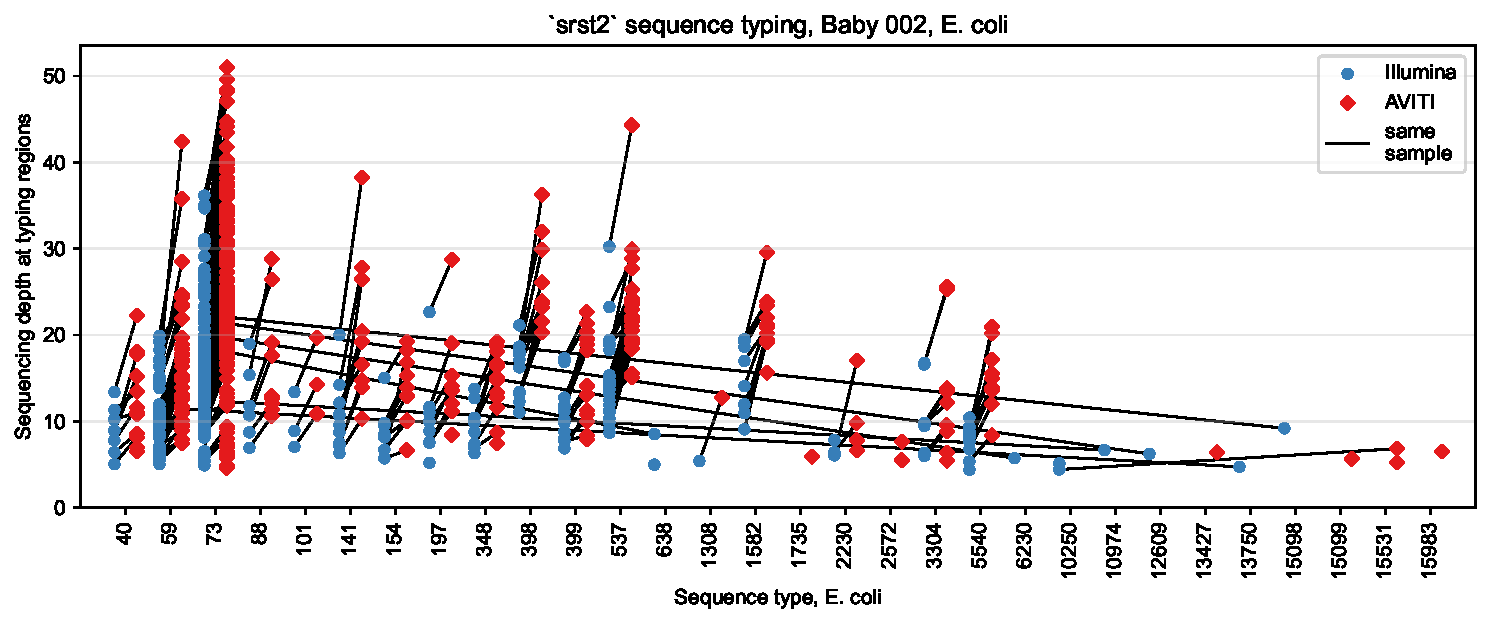
\includegraphics[width=.95\textwidth]{figures/sequence_typing.pdf}
    \caption{
        \textbf{Sequence typing results} for successful \texttt{srst2} sequence typing of identical samples ($-$) 
        prepared using \textcolor{red}{AVITI} (\textcolor{red}{$\diamond$}) or \textcolor{blue}{Illumina} (\textcolor{blue}{$\bullet$}).
    }
    \label{figure:st}
\end{figure}

\begin{table}[h]
    \centering
    \begin{tabular}{lr}
\toprule
 & Count \\
\midrule
AVITI \& Illumina (total) & 398 \\
AVITI, typed (total) & 379 \\
Illumina, typed (total) & 331 \\
AVITI \& Illumina, typed (total) & 312 \\
AVITI \& Illumina, typed (agree) & 305 \\
\bottomrule
\end{tabular}

    \caption{
        \textbf{Summary of sequence typing results}, tallying the number of samples for different criteria. 
        The top row provides the total number of samples; 
        the bottom row provides the number of samples \textit{successfully} sequence typed for \textit{both} AVITI \textit{and} Illumina 
        \textit{and agree} in the designated sequence type.
    }
    \label{tab:st}
\end{table}


\section{Reconstructing phylogenies of dominant STs}

\section{Appendix}

Code to reproduce is available on GitHub at \href{https://github.com/t-silvers/sequencing-comparison-aviti-illumina}{t-silvers/sequencing-comparison-aviti-illumina}.

\end{document}